\documentclass{beamer}

\usetheme{CambridgeUS}
\usecolortheme{orchid}

\usepackage[utf8]{inputenc}
\usepackage[T1]{fontenc}

% Paths
\newcommand{\figs}{../figs}
\newcommand{\data}{../data}
\newcommand{\code}{../code}

% URL styles
\usepackage{url}
\urlstyle{sf}

% Units
\usepackage[detect-weight=true, binary-units=true]{siunitx}
\DeclareSIUnit\flop{Flops}

% Math
\usepackage{amsmath}
\usepackage{amssymb}
\usepackage{bm}
\usepackage{nicefrac}
\newcommand{\dif}[1]{{\;\text{d}#1}}

% Graphics
\usepackage{graphicx}
\usepackage{caption}
\usepackage{subcaption}
\graphicspath{{../figs/}}

% Tikz
\usepackage{tikz}
\usetikzlibrary{positioning,shapes,arrows,calc,intersections}
\usepackage{pgfplots}
\usepgfplotslibrary{dateplot}
\pgfplotsset{compat=1.8}

% Colors
\definecolor{darkblue}{HTML}{00688B}
\definecolor{darkgreen}{HTML}{6E8B3D}
\definecolor{cadet}{HTML}{DAE1FF}
\definecolor{salmon}{HTML}{FFB08A}

% Listings
\usepackage{textcomp}
\usepackage{listings}
\lstset{
  keywordstyle=\bfseries\color{orange},
  stringstyle=\color{darkblue!80},
  commentstyle=\color{darkblue!80},
  showstringspaces=false,
  basicstyle=\ttfamily,
  upquote=true,
}
\lstdefinestyle{fortran}{
  language=Fortran,
  morekeywords={for},
  deletekeywords={status},
}
\lstdefinestyle{c}{
  language=C,
  morekeywords={include},
}
\lstdefinestyle{glsl}{
  language=C,
  morekeywords={attribute, vec2, vec3, vec4, varying, uniform, mat2, mat3, mat4},
}
\lstdefinestyle{cuda}{
  language=C,
  morekeywords={__global__, __device__, __host__},
}
\lstdefinestyle{shell}{
  language=bash,
  morekeywords={mkdir, ssh, cmake},
}

% Double hlines
\usepackage{hhline}

% Misc
\usepackage{nth}

\subtitle{TMA4280---Introduction to Supercomputing}

\begin{document}


\title{Curriculum}
\author{Eivind Fonn}
\institute{SINTEF ICT / NTNU}
\date{December 2015}
\maketitle

\begin{frame}
  \frametitle{Supercomputer history and hardware architecture}
  \begin{center}
    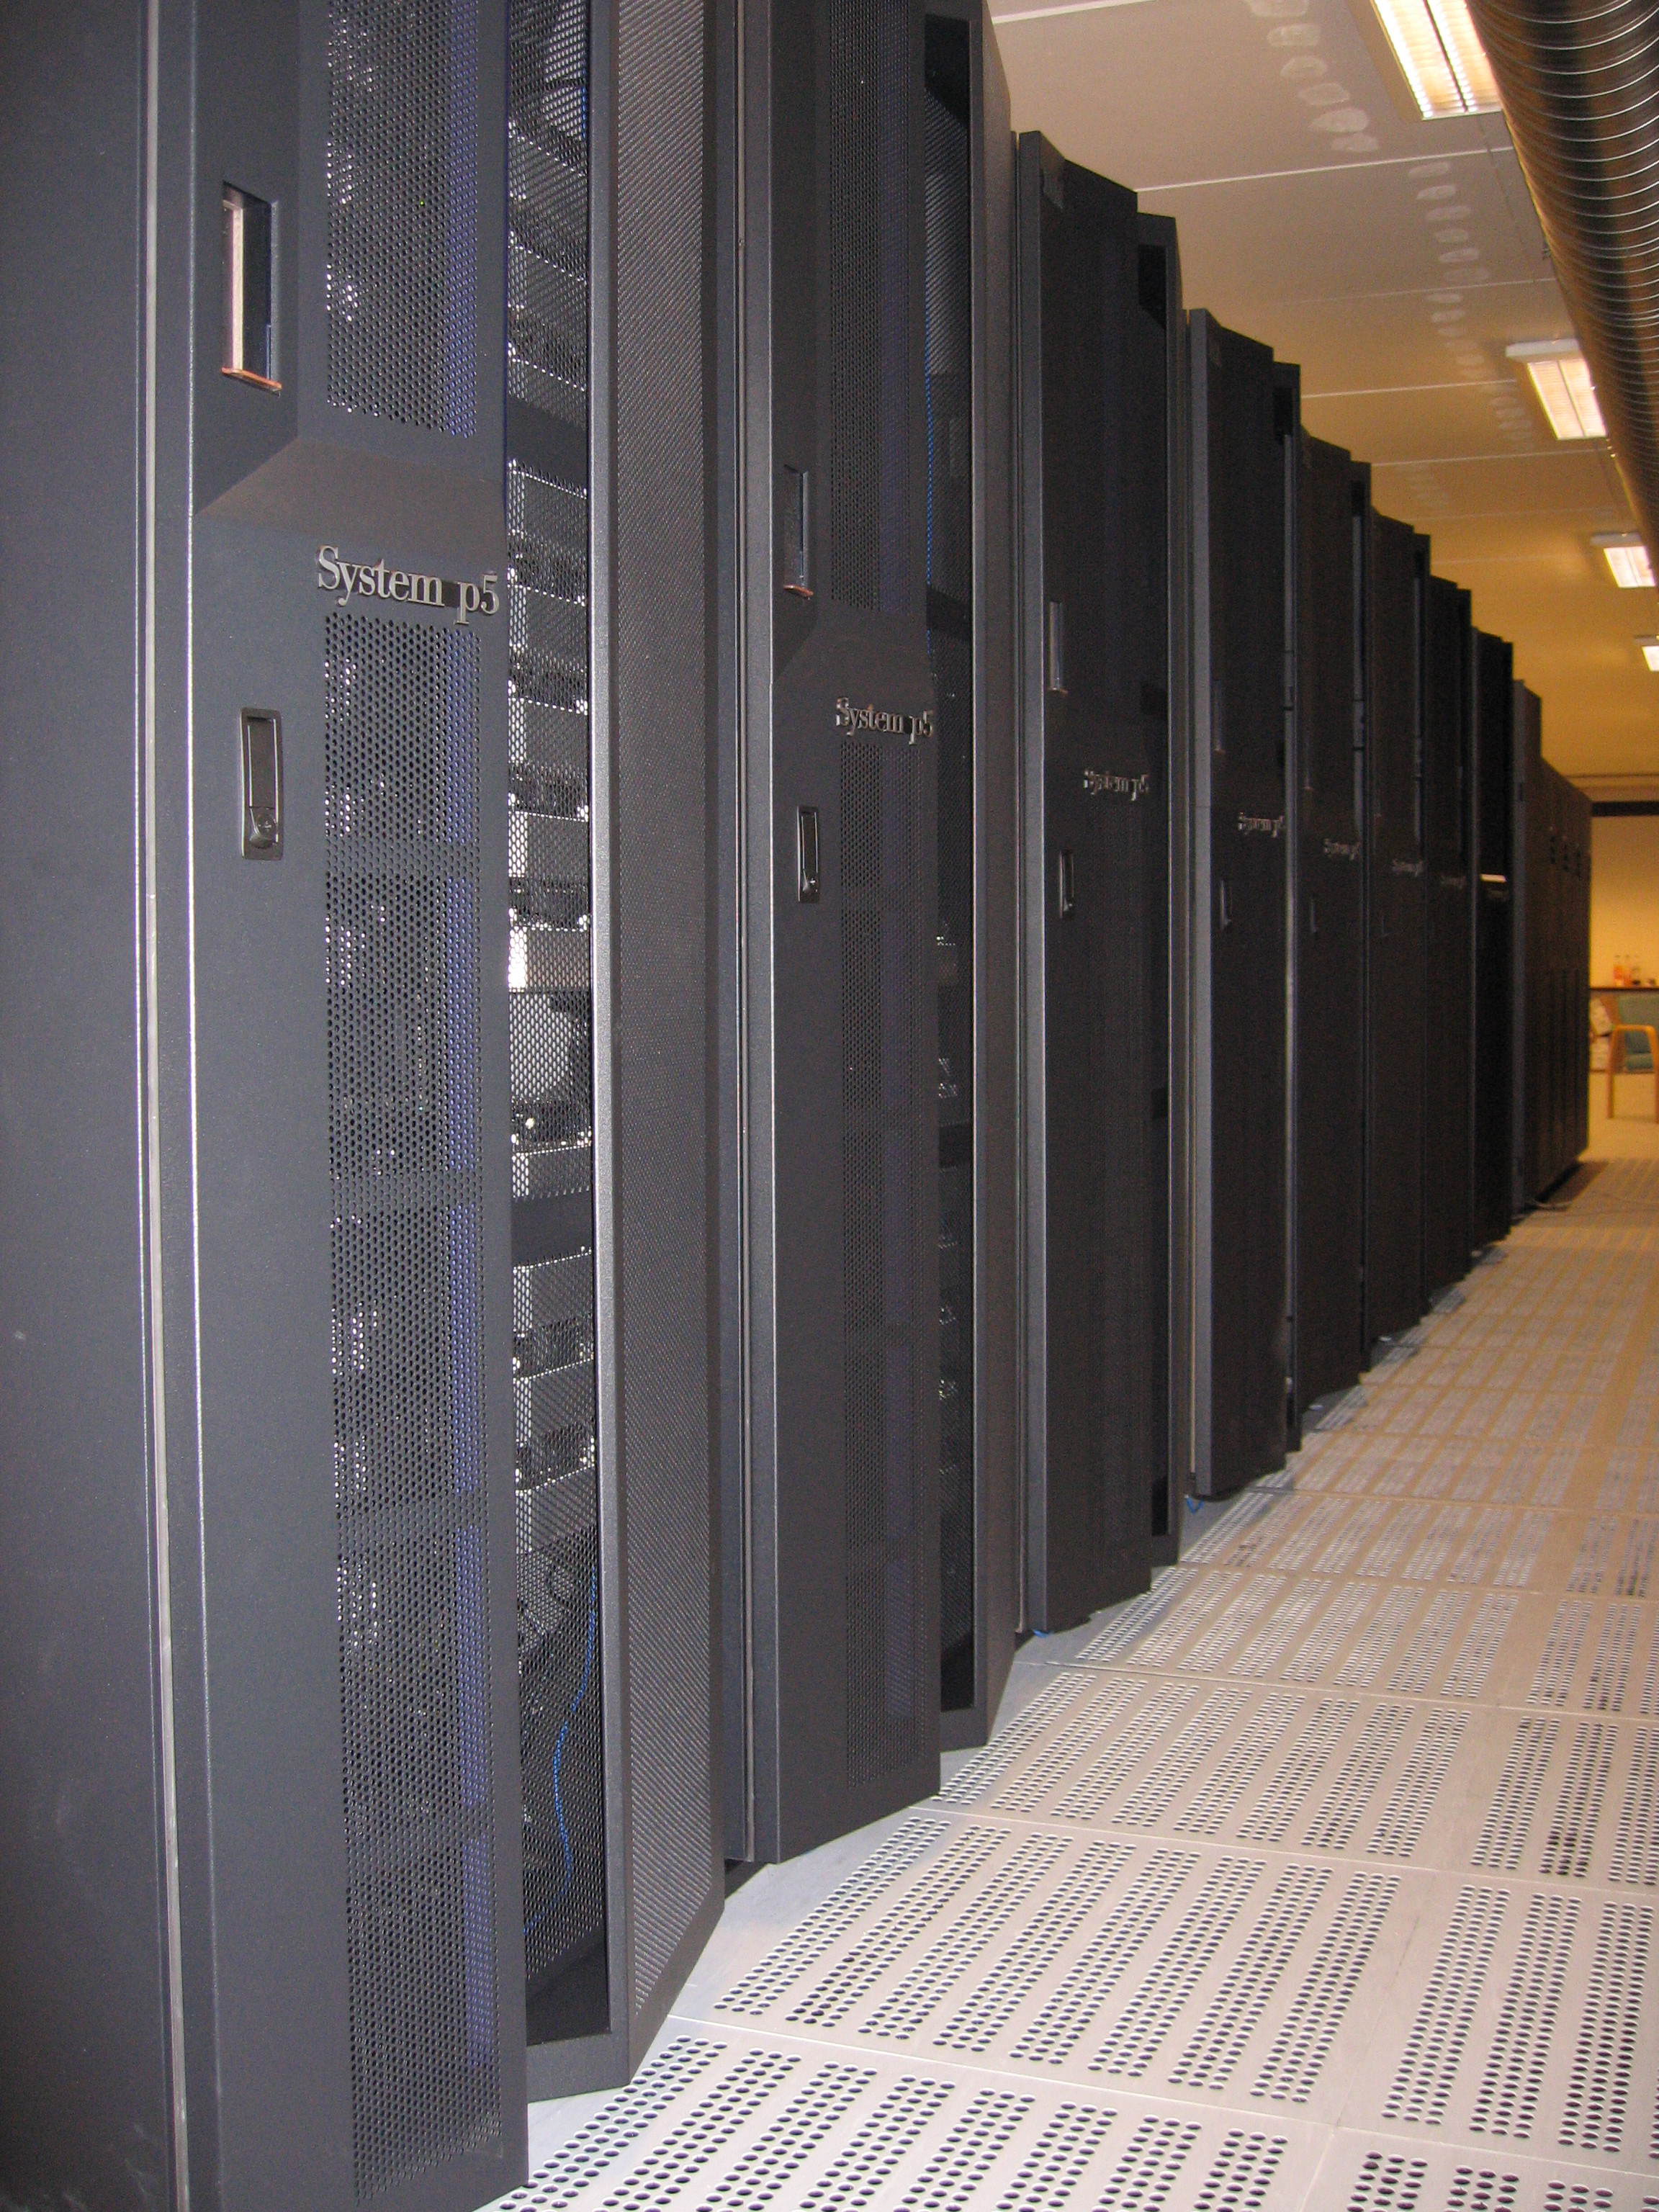
\includegraphics[height=0.6\textheight]{njord_1}
  \end{center}
\end{frame}

\begin{frame}
  \frametitle{An UNIX crash course---ssh, bash, build systems (CMake)}
  \begin{center}
    
\includegraphics[width=6cm]{crash}
  \end{center}
\end{frame}

\begin{frame}[fragile]
  \frametitle{Distributed memory programming with MPI}
  \begin{center}
    \texttt{node 0: Hello, world} \\
    \texttt{node 1: Hello, world} \\
    \texttt{node 3: Hello, world} \\
    \texttt{node 2: Hello, world}
  \end{center}
  \begin{center}
    
\includegraphics[width=3cm]{open-mpi-logo}
  \end{center}
\end{frame}

\begin{frame}
  \frametitle{Shared memory programming with OpenMP}
  \begin{center}
    \texttt{\#pragma omp parallel for schedule(static)}
  \end{center}
  \begin{center}
    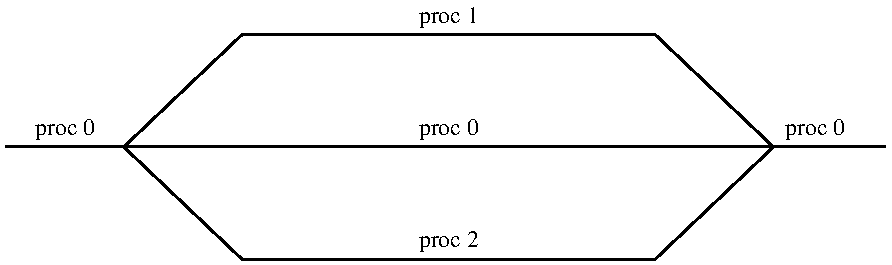
\includegraphics[width=4cm]{openmp}
  \end{center}
\end{frame}

% \begin{frame}
%   \frametitle{Heterogeneous computing with CUDA}
%   \begin{center}
%     \texttt{int row = blockIdx.x*blockDim.x+threadIdx.x;}
%   \end{center}
%   \begin{center}
%     
\includegraphics[width=4cm]{cuda}
%   \end{center}
% \end{frame}

\begin{frame}
  \frametitle{Poisson problem: finite differences}
  \[
    \begin{split}
      -\nabla^2 u &= f \\
      u_{\partial\Omega} &= g
    \end{split}
  \]
  \begin{center}
    \scalebox{0.8}{
      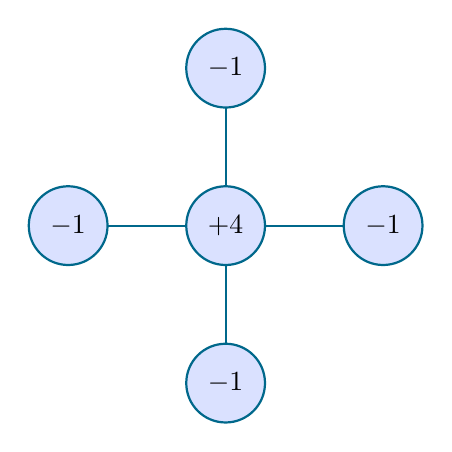
\begin{tikzpicture}[
  every node/.style={
    shape=circle,
    thick,
    fill=cadet,
    draw=darkblue,
    minimum size=1cm,
  }]
  \draw[thick, darkblue] (-2,0) -- (2,0);
  \draw[thick, darkblue] (0,-2) -- (0,2);
  \node at (-2,0) {$-1$};
  \node at (2,0) {$-1$};
  \node at (0,-2) {$-1$};
  \node at (0,2) {$-1$};
  \node at (0,0) {$+4$};
\end{tikzpicture}

    }
  \end{center}
\end{frame}

\begin{frame}
  \frametitle{Poisson problem: Diagonalization methods}
  \begin{enumerate}
  \item Compute $\tilde{\bm G}$ using matrix-matrix products
    \begin{equation*}
      \tilde{\bm G} = \bm Q^\intercal \bm G \bm Q.
    \end{equation*}
  \item Solve for $\tilde{\bm U}$.
    \begin{align*}
      \bm \Lambda \tilde{\bm U} + \tilde{\bm U} \bm \Lambda &= \tilde{\bm G} \\
      \lambda_i \tilde{u}_{ij} + \tilde{u}_{ij} \lambda_j &= \tilde{g}_{ij} \\
      \tilde{u}_{ij} &= \frac{\tilde{g}_{ij}}{\lambda_i + \lambda_j}
    \end{align*}
  \item Compute $\bm U$ using matrix-matrix products
    \begin{equation*}
      \bm U = \bm Q \tilde{\bm U} \bm Q^\intercal
    \end{equation*}
  \end{enumerate}
\end{frame}

\begin{frame}
  \frametitle{The conjugate gradient method}
  \begin{center}
    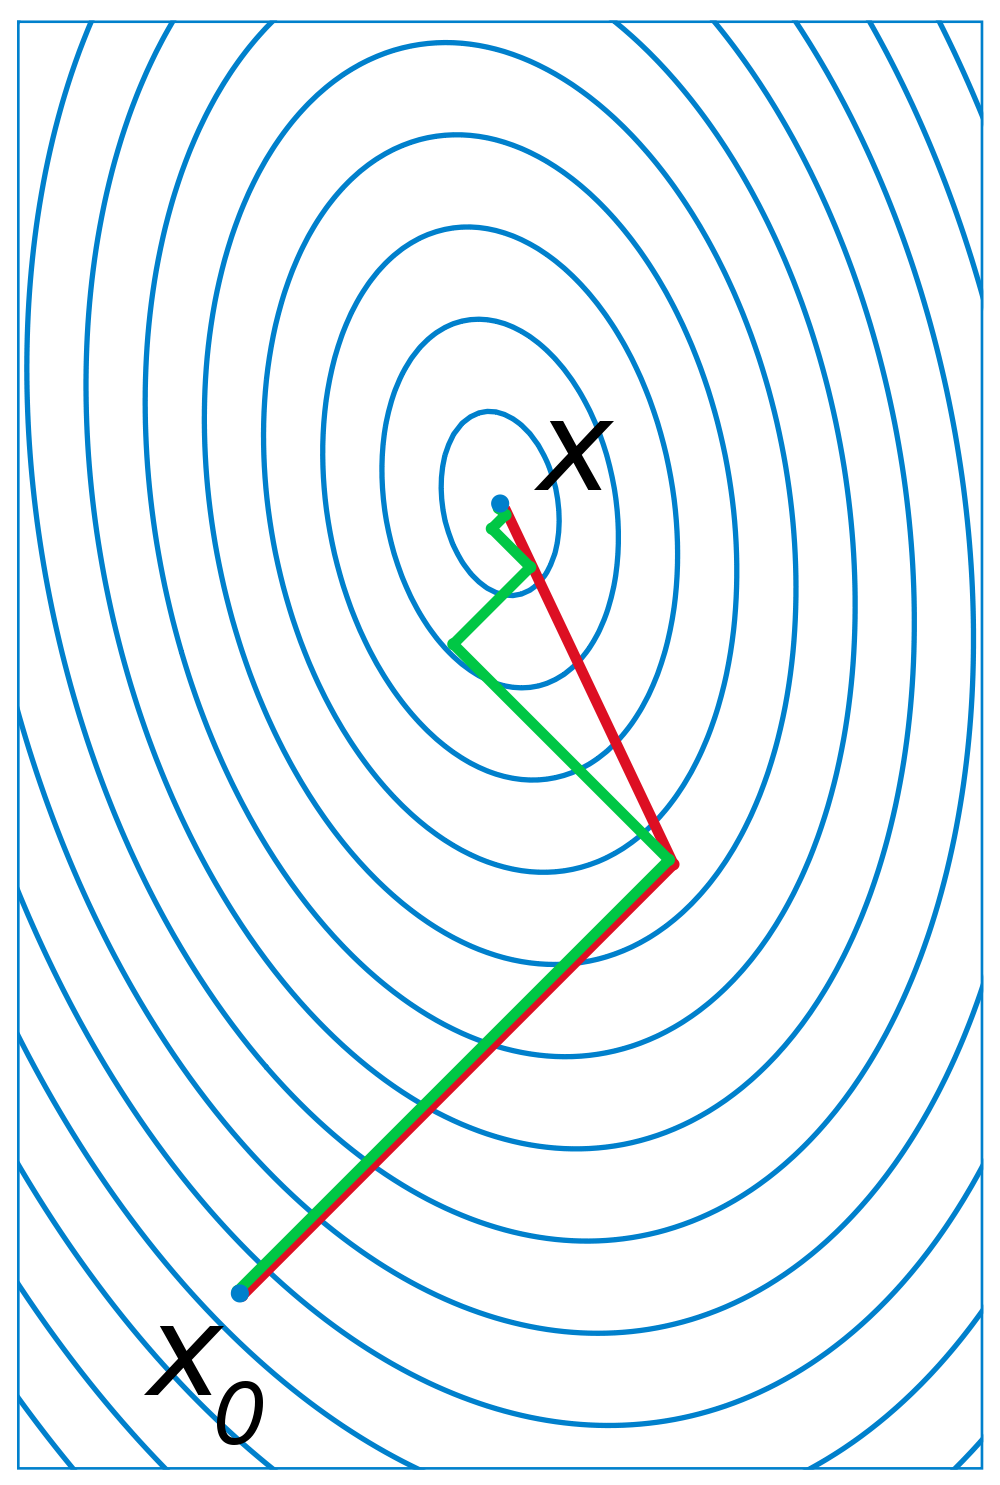
\includegraphics[width=4cm]{cg}
  \end{center}
\end{frame}

\begin{frame}
  \frametitle{Poisson problem: Domain decomposition}
  \begin{center}
    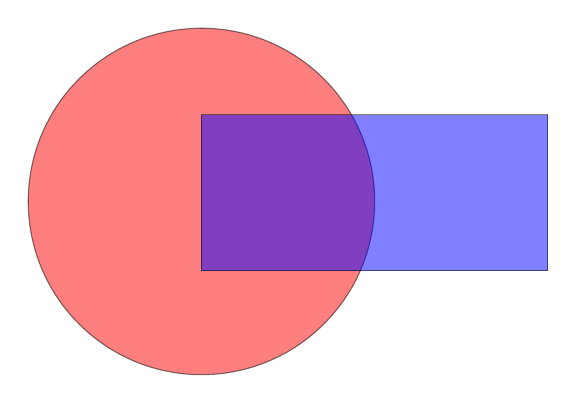
\begin{tikzpicture}[scale=2.2]
      \draw[black, fill=red, opacity=0.5] (0,0) circle (1);
      \draw[black, fill=blue, opacity=0.5] (0,-0.4) rectangle (2,0.5);
    \end{tikzpicture}
  \end{center}
\end{frame}

\begin{frame}
  \frametitle{Parallell I/O with MPI-IO}
  \begin{center}
    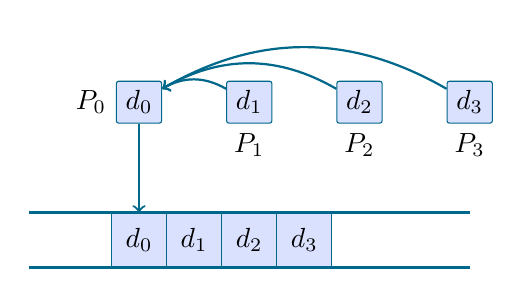
\begin{tikzpicture}[
      scale=0.7,
      data/.style={
        rectangle,
        draw=darkblue,
        fill=cadet,
        rounded corners=0.8,
      }
      ]
      \node[data] (d0) at (0,0) {$d_0$};
      \node[data] (d1) at (2,0) {$d_1$};
      \node[data] (d2) at (4,0) {$d_2$};
      \node[data] (d3) at (6,0) {$d_3$};
      \node[left=0.0 of d0.west] {$P_0$};
      \node[below=0.0 of d1.south] {$P_1$};
      \node[below=0.0 of d2.south] {$P_2$};
      \node[below=0.0 of d3.south] {$P_3$};
      \draw[->, darkblue, thick] (d1) edge[bend right] node [above] {} (d0);
      \draw[->, darkblue, thick] (d2) edge[bend right] node [above] {} (d0);
      \draw[->, darkblue, thick] (d3) edge[bend right] node [above] {} (d0);
      \foreach \i in {0,...,3} {
        \draw[darkblue, fill=cadet] (-0.5+\i, -3) rectangle (0.5+\i, -2);
        \node at (\i, -2.5) {$d_\i$};
      }
      \draw[darkblue, thick] (-2, -3) -- (6, -3);
      \draw[darkblue, thick] (-2, -2) -- (6, -2);
      \draw[darkblue, thick, ->] (d0.south) -- (0,-2);
    \end{tikzpicture}
  \end{center}
\end{frame}

\end{document}

